\documentclass{beamer}
\usepackage[latin1]{inputenc}
%\usetheme{Montpellier}
\usetheme{Boadilla}
%\usecolortheme[RGB={204,51,255}]{structure}
%\usecolortheme[named=purple]{structure}
\usecolortheme[RGB={62,128,62}]{structure}
%\definecolor{dark}{rgb}{0.4,0.20,0.4}
%\definecolor{light}{rgb}{0.8,0.6,0.8}
%\definecolor{reddish}{rgb}{.5,0.15,0.15}
\definecolor{dark}{rgb}{0.55,0.35,0.45}
%\definecolor{light}{rgb}{0.8,0.6,0.8}
\definecolor{reddish}{rgb}{.7,0.25,0.25}
\usepackage{graphicx}
\usepackage{pstricks}

\usepackage{tikz}
\usetikzlibrary{arrows,decorations.markings,positioning}
\usepackage{epstopdf}
\newcommand{\btVFill}{\vskip0pt plus 1filll}

\title[A Kozachenko-Leonenko estimator.]{Mutual information on metric spaces.}
\author{Conor Houghton}
\institute{CS, U Bristol}
\date{Bayesian Workshop, 2019}

\begin{document}

\maketitle

\begin{frame}{Outline}
This talk will be about estimating mutual information on metric spaces.
\begin{itemize}
\item I became interested in this topic because of the application to spike trains.
\item I believe that the approach outlined here has applications elsewhere, perhaps in machine learning.
\end{itemize}
\color{black}
\end{frame}

\begin{frame}{Neurons}
\color{reddish}
\begin{center}
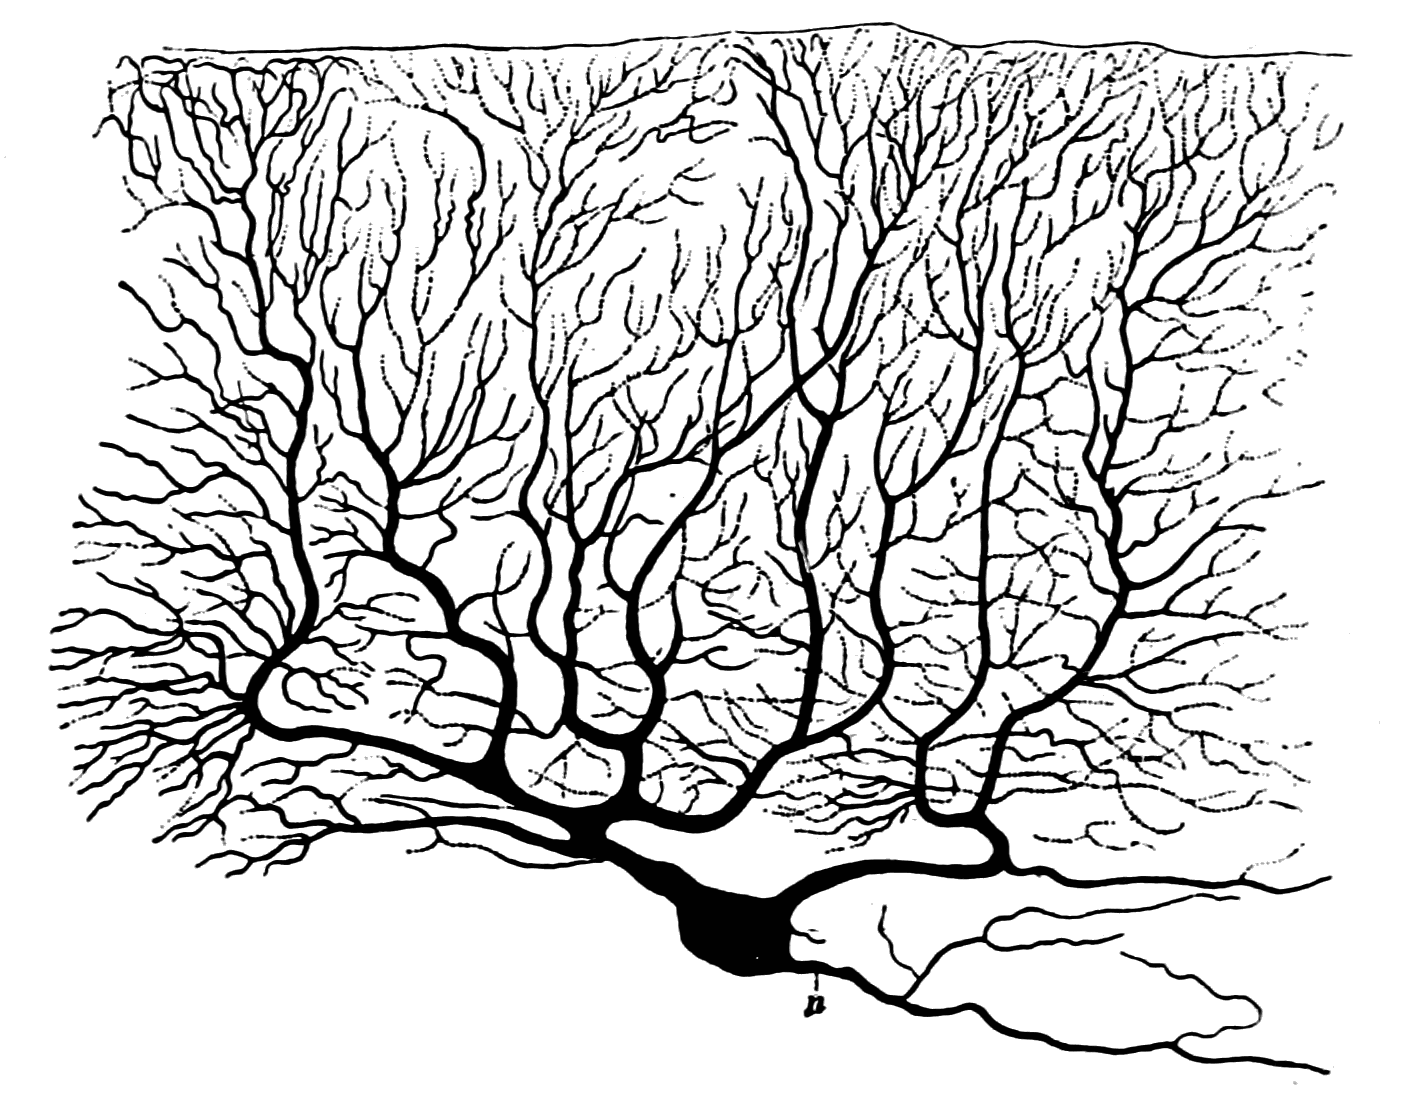
\includegraphics[width=8cm]{PC.png}
\end{center}
\btVFill
\begin{flushright}
\tiny{Picture from wikisource.}
\end{flushright}
\end{frame}

\begin{frame}{Spikes}
\color{reddish}
\begin{center}
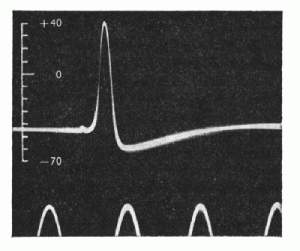
\includegraphics[width=8cm]{spike.png}
\end{center}
\btVFill
\begin{flushright}
\tiny{Picture from Hodgkin and Huxley, 1939.}
\end{flushright}
\end{frame}



\begin{frame}{Spike trains}
\color{reddish}
\begin{center}
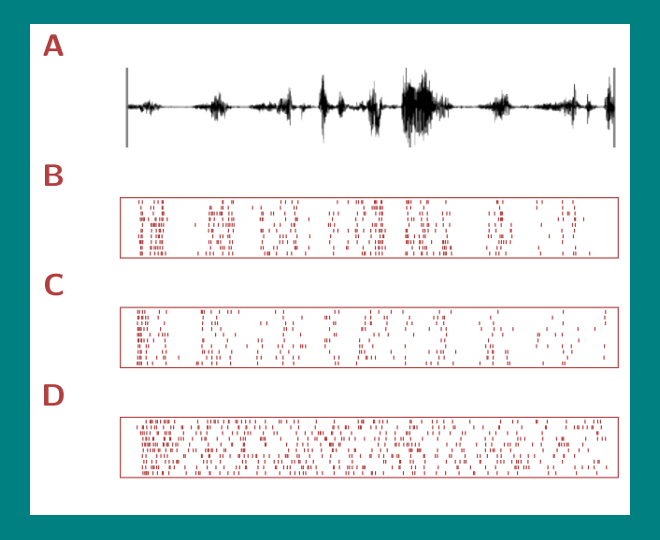
\includegraphics[width=8cm]{SpikeTrains.png}
\end{center}
\end{frame}


\begin{frame}{Shannon's entropy}
\color{dark}
$$
H(X)=-\sum_x p(x)\log_2{p(x)}
$$
\color{black}
\end{frame}



\begin{frame}{Shannon's entropy}
\color{dark}
$$
H(X)=-\sum_x p(x)\log_2{p(x)}
$$
\color{black}
\begin{center}
\begin{tabular}{cccccccc}
A& B& C& D& E& F& G& H\\
1/2&1/4&1/8&1/16&1/32&1/64&1/128&1/128\\
000&001&010&011&100&101&110&111\\
0&10&110&1110&11110&111110&1111110&1111111
\end{tabular}
\end{center}
\color{dark}
$$
\mbox{average code length}=\frac{1}{2}+\frac{1}{4}2+\frac{1}{8}3+\frac{1}{16}4+\ldots = H(X)\approx 1.98 < 3
$$
\color{black}
\end{frame}

\begin{frame}{Conditional entropy}
\color{dark}
  $$
H(X|S=s)=-\sum_x p(x|s)\log_2{p(x|s)}
$$
\color{black}
and
\color{dark}
$$
H(X|S)=H(X|S)=\langle H(X|s)\rangle_s
$$
\color{black}
If $X$ is the stimulus $H(X|S)$ quantifies noise.
\end{frame}


\begin{frame}{Differential entropy}
  \color{dark}
$$
H(X)=-\int dx p_X(x)\log_2 {p_X(x)}
$$
\end{frame}



\begin{frame}{Differential entropy is tricky}
  \color{dark}
$$
H(X)=-\int dx p_X(x)\log_2 {p_X(x)}
$$
\color{black}
If $y=\lambda x$ we have
\color{dark}
$$p_X(x)dx=p_Y(y)dy$$
\color{black}
but
\color{dark}
$$
p_Y(y)=p_X(x)/\lambda
$$
\color{black}
so
\color{dark}
$$
H(Y)= H(X)+\log_2{\lambda}
$$

\end{frame}

\begin{frame}{Mutual information}
\color{dark}
$$
I(X,Y)=\sum_{x,y} p_{X,Y}(x,y) \log_2{\frac{p_{X,Y}(x,y)}{p_X(x)p_Y(y)}}
$$
\color{black}
\end{frame}


\begin{frame}{Mutual information}
\color{dark}
$$
I(X,Y)=\sum_{x,y} p_{X,Y}(x,y) \log_2{\frac{p_{X,Y}(x,y)}{p_X(x)p_Y(y)}}
$$
\color{black}
gives
\color{dark}
$$
I(X,Y)=H(X)-H(X|Y)=H(Y)-H(Y|X)
$$
\color{black}
\end{frame}


\begin{frame}{Mutual information}
\color{dark}
$$
I(X,Y)=H(X)-H(X|Y)=H(Y)-H(Y|X)
$$
\color{black}
\vskip 1 cm
so, for example
\color{dark}
$$
H(Y)=H(Y|X)+I(X,Y)
$$
\color{black}
\begin{center}
info in $Y$=(info remaining in Y if you know X)+(mutual info)
\end{center}
\end{frame}



\begin{frame}{Spike trains again}
\color{reddish}
\begin{center}
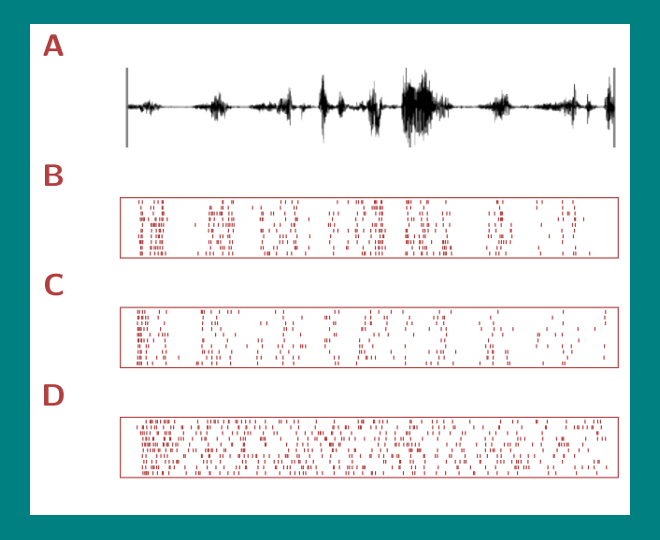
\includegraphics[width=8cm]{SpikeTrains.png}
\end{center}
\end{frame}


\begin{frame}{Classical approach}
\begin{itemize}
\item Discretize.
\color{reddish}
\begin{center}
\setlength{\unitlength}{1000sp}%
%
\begingroup\makeatletter\ifx\SetFigFont\undefined%
\gdef\SetFigFont#1#2#3#4#5{%
  \reset@font\fontsize{#1}{#2pt}%
  \fontfamily{#3}\fontseries{#4}\fontshape{#5}%
  \selectfont}%
\fi\endgroup%
\begin{picture}(6793,2767)(1789,-5945)
\thinlines
{\color[rgb]{0,0,0}\put(1801,-4111){\line( 1, 0){6750}}
}%
\thicklines
{\color[rgb]{0,0,0}\put(4276,-3211){\line( 0,-1){900}}
}%
{\color[rgb]{0,0,0}\put(7381,-3211){\line( 0,-1){900}}
}%
{\color[rgb]{0,0,0}\put(2521,-3211){\line( 0,-1){900}}
}%
\thinlines
{\color[rgb]{0,0,0}\put(2251,-5821){\line( 0,-1){ 90}}
}%
{\color[rgb]{0,0,0}\put(2701,-5821){\line( 0,-1){ 90}}
}%
{\color[rgb]{0,0,0}\put(3151,-5821){\line( 0,-1){ 90}}
}%
{\color[rgb]{0,0,0}\put(4051,-5821){\line( 0,-1){ 90}}
}%
{\color[rgb]{0,0,0}\put(4501,-5821){\line( 0,-1){ 90}}
}%
{\color[rgb]{0,0,0}\put(4951,-5821){\line( 0,-1){ 90}}
}%
{\color[rgb]{0,0,0}\put(5401,-5821){\line( 0,-1){ 90}}
}%
{\color[rgb]{0,0,0}\put(5851,-5821){\line( 0,-1){ 90}}
}%
{\color[rgb]{0,0,0}\put(6301,-5821){\line( 0,-1){ 90}}
}%
{\color[rgb]{0,0,0}\put(6751,-5821){\line( 0,-1){ 90}}
}%
{\color[rgb]{0,0,0}\put(7201,-5821){\line( 0,-1){ 90}}
}%
{\color[rgb]{0,0,0}\put(7651,-5821){\line( 0,-1){ 90}}
}%
{\color[rgb]{0,0,0}\put(8101,-5821){\line( 0,-1){ 90}}
}%
{\color[rgb]{0,0,0}\put(8551,-5821){\line( 0,-1){ 90}}
}%
\thicklines
{\color[rgb]{0,0,0}\put(5176,-4336){\vector( 0,-1){900}}
}%
\thinlines
{\color[rgb]{0,0,0}\put(1803,-5843){\line( 0,-1){ 90}}
}%
{\color[rgb]{0,0,0}\put(1820,-5916){\line( 1, 0){6750}}
}%
{\color[rgb]{0,0,0}\put(3603,-5814){\line( 0,-1){ 90}}
}%
\put(1858,-5871){\makebox(0,0)[lb]{0}}%
\put(2308,-5871){\makebox(0,0)[lb]{1}}%
\put(2758,-5871){\makebox(0,0)[lb]{0}}%
\put(3208,-5871){\makebox(0,0)[lb]{0}}%
\put(3658,-5871){\makebox(0,0)[lb]{0}}%
\put(4108,-5871){\makebox(0,0)[lb]{1}}%
\put(4558,-5871){\makebox(0,0)[lb]{0}}%
\put(5008,-5871){\makebox(0,0)[lb]{0}}%
\put(5458,-5871){\makebox(0,0)[lb]{0}}%
\put(5908,-5871){\makebox(0,0)[lb]{0}}%
\put(6358,-5871){\makebox(0,0)[lb]{0}}%
\put(6808,-5871){\makebox(0,0)[lb]{0}}%
\put(7258,-5871){\makebox(0,0)[lb]{1}}%
\put(7708,-5871){\makebox(0,0)[lb]{0}}%
\put(8158,-5871){\makebox(0,0)[lb]{0}}%
\end{picture}%

\end{center}
\color{black}
\item Split into words.
\color{dark}
$$010001000000100\rightarrow 01000,10000,00100$$
\color{black}
\end{itemize}
\btVFill
\begin{flushright}
\tiny{Bialek, de Ruyer van Steveninck, Strong and other coworkers, late 1990s.}
\end{flushright}
\end{frame}

\begin{frame}{Classical approach}
\begin{itemize}
\item Estimate probability of words. For example, say $w_8=01000$ then estimate
\color{dark}
$$p(w_8)\approx\frac{\#\mbox{ occurrences of }w_8}{\#\mbox{ words}}$$ 
\color{black}
\item Calculate
\color{dark}
$$H(W)=-\sum_i p(w_i)\log_2 p(w_i) =-\langle\log_2 p(w_i)\rangle$$ 
\color{black}
\end{itemize}
\btVFill
\begin{flushright}
\tiny{Bialek, de Ruyer van Steveninck, Strong and other coworkers, late 1990s.}
\end{flushright}
\end{frame}


\begin{frame}{Classical approach}
\begin{itemize}
\item Conditional probability.
\color{reddish}
\begin{center}
\setlength{\unitlength}{1000sp}%
%
\begingroup\makeatletter\ifx\SetFigFont\undefined%
\gdef\SetFigFont#1#2#3#4#5{%
  \reset@font\fontsize{#1}{#2pt}%
  \fontfamily{#3}\fontseries{#4}\fontshape{#5}%
  \selectfont}%
\fi\endgroup%
\begin{picture}(14000,7000)(1789,-7945)

\thinlines
{\color[rgb]{0,0,0}\put(2251,-5821){\line( 0,-1){ 90}}
}%
{\color[rgb]{0,0,0}\put(2701,-5821){\line( 0,-1){ 90}}
}%
{\color[rgb]{0,0,0}\put(3151,-5821){\line( 0,-1){ 90}}
}%
{\color[rgb]{0,0,0}\put(4051,-5421){\line( 0,-1){490}}
}%
{\color[rgb]{0,0,0}\put(4501,-5821){\line( 0,-1){ 90}}
}%
{\color[rgb]{0,0,0}\put(4951,-5821){\line( 0,-1){90}}
}%
{\color[rgb]{0,0,0}\put(5401,-5821){\line( 0,-1){ 90}}
}%
{\color[rgb]{0,0,0}\put(5851,-5821){\line( 0,-1){ 90}}
}%
{\color[rgb]{0,0,0}\put(6301,-5421){\line( 0,-1){490}}
}%
{\color[rgb]{0,0,0}\put(6751,-5821){\line( 0,-1){ 90}}
}%
{\color[rgb]{0,0,0}\put(7201,-5821){\line( 0,-1){ 90}}
}%
{\color[rgb]{0,0,0}\put(7651,-5821){\line( 0,-1){ 90}}
}%
{\color[rgb]{0,0,0}\put(8101,-5821){\line( 0,-1){ 90}}
}%
{\color[rgb]{0,0,0}\put(8551,-5421){\line( 0,-1){490}}
}%
{\color[rgb]{0,0,0}\put(9001,-5821){\line( 0,-1){ 90}}
}%
{\color[rgb]{0,0,0}\put(9451,-5821){\line( 0,-1){ 90}}
}%
{\color[rgb]{0,0,0}\put(9901,-5821){\line( 0,-1){ 90}}
}%
{\color[rgb]{0,0,0}\put(10351,-5821){\line( 0,-1){ 90}}
}%
{\color[rgb]{0,0,0}\put(10801,-5421){\line( 0,-1){ 490}}
}%
{\color[rgb]{0,0,0}\put(11251,-5821){\line( 0,-1){ 90}}
}%
{\color[rgb]{0,0,0}\put(11701,-5821){\line( 0,-1){ 90}}
}%
{\color[rgb]{0,0,0}\put(12151,-5821){\line( 0,-1){ 90}}
}%
{\color[rgb]{0,0,0}\put(12601,-5821){\line( 0,-1){ 90}}
}%
{\color[rgb]{0,0,0}\put(13051,-5421){\line( 0,-1){ 490}}
}%
{\color[rgb]{0,0,0}\put(13501,-5821){\line( 0,-1){ 90}}
}%
{\color[rgb]{0,0,0}\put(13951,-5821){\line( 0,-1){ 90}}
}%
{\color[rgb]{0,0,0}\put(14401,-5821){\line( 0,-1){ 90}}
}%
{\color[rgb]{0,0,0}\put(14851,-5821){\line( 0,-1){ 90}}
}%
{\color[rgb]{0,0,0}\put(15301,-5421){\line( 0,-1){490}}
}%
{\color[rgb]{0,0,0}\put(1803,-5421){\line( 0,-1){ 490}}
}%
{\color[rgb]{0,0,0}\put(1820,-5916){\line( 1, 0){13481}}
}%
{\color[rgb]{0,0,0}\put(3603,-5814){\line( 0,-1){ 90}}
}%
\put(1858,-5871){\makebox(0,0)[lb]{0}}%
\put(2308,-5871){\makebox(0,0)[lb]{0}}%
\put(2758,-5871){\makebox(0,0)[lb]{1}}%
\put(3208,-5871){\makebox(0,0)[lb]{0}}%
\put(3658,-5871){\makebox(0,0)[lb]{0}}%
\put(4108,-5871){\makebox(0,0)[lb]{1}}%
\put(4558,-5871){\makebox(0,0)[lb]{0}}%
\put(5008,-5871){\makebox(0,0)[lb]{0}}%
\put(5458,-5871){\makebox(0,0)[lb]{1}}%
\put(5908,-5871){\makebox(0,0)[lb]{0}}%
\put(6358,-5871){\makebox(0,0)[lb]{0}}%
\put(6808,-5871){\makebox(0,0)[lb]{0}}%
\put(7258,-5871){\makebox(0,0)[lb]{0}}%
\put(7708,-5871){\makebox(0,0)[lb]{1}}%
\put(8158,-5871){\makebox(0,0)[lb]{0}}%
\put(8608,-5871){\makebox(0,0)[lb]{0}}%
\put(9058,-5871){\makebox(0,0)[lb]{1}}%
\put(9508,-5871){\makebox(0,0)[lb]{0}}%
\put(9958,-5871){\makebox(0,0)[lb]{0}}%
\put(10408,-5871){\makebox(0,0)[lb]{0}}%
\put(10858,-5871){\makebox(0,0)[lb]{1}}%
\put(11308,-5871){\makebox(0,0)[lb]{0}}%
\put(11758,-5871){\makebox(0,0)[lb]{1}}%
\put(12208,-5871){\makebox(0,0)[lb]{0}}%
\put(12658,-5871){\makebox(0,0)[lb]{0}}%
\put(13108,-5871){\makebox(0,0)[lb]{1}}%
\put(13558,-5871){\makebox(0,0)[lb]{0}}%
\put(14008,-5871){\makebox(0,0)[lb]{0}}%
\put(14458,-5871){\makebox(0,0)[lb]{0}}%
\put(14908,-5871){\makebox(0,0)[lb]{0}}%


\thinlines
{\color[rgb]{0,0,0}\put(2251,-4821){\line( 0,-1){ 90}}
}%
{\color[rgb]{0,0,0}\put(2701,-4821){\line( 0,-1){ 90}}
}%
{\color[rgb]{0,0,0}\put(3151,-4821){\line( 0,-1){ 90}}
}%
{\color[rgb]{0,0,0}\put(4051,-4421){\line( 0,-1){490}}
}%
{\color[rgb]{0,0,0}\put(4501,-4821){\line( 0,-1){ 90}}
}%
{\color[rgb]{0,0,0}\put(4951,-4821){\line( 0,-1){90}}
}%
{\color[rgb]{0,0,0}\put(5401,-4821){\line( 0,-1){ 90}}
}%
{\color[rgb]{0,0,0}\put(5851,-4821){\line( 0,-1){ 90}}
}%
{\color[rgb]{0,0,0}\put(6301,-4421){\line( 0,-1){490}}
}%
{\color[rgb]{0,0,0}\put(6751,-4821){\line( 0,-1){ 90}}
}%
{\color[rgb]{0,0,0}\put(7201,-4821){\line( 0,-1){ 90}}
}%
{\color[rgb]{0,0,0}\put(7651,-4821){\line( 0,-1){ 90}}
}%
{\color[rgb]{0,0,0}\put(8101,-4821){\line( 0,-1){ 90}}
}%
{\color[rgb]{0,0,0}\put(8551,-4421){\line( 0,-1){490}}
}%
{\color[rgb]{0,0,0}\put(9001,-4821){\line( 0,-1){ 90}}
}%
{\color[rgb]{0,0,0}\put(9451,-4821){\line( 0,-1){ 90}}
}%
{\color[rgb]{0,0,0}\put(9901,-4821){\line( 0,-1){ 90}}
}%
{\color[rgb]{0,0,0}\put(10351,-4821){\line( 0,-1){ 90}}
}%
{\color[rgb]{0,0,0}\put(10801,-4421){\line( 0,-1){ 490}}
}%
{\color[rgb]{0,0,0}\put(11251,-4821){\line( 0,-1){ 90}}
}%
{\color[rgb]{0,0,0}\put(11701,-4821){\line( 0,-1){ 90}}
}%
{\color[rgb]{0,0,0}\put(12151,-4821){\line( 0,-1){ 90}}
}%
{\color[rgb]{0,0,0}\put(12601,-4821){\line( 0,-1){ 90}}
}%
{\color[rgb]{0,0,0}\put(13051,-4421){\line( 0,-1){ 490}}
}%
{\color[rgb]{0,0,0}\put(13501,-4821){\line( 0,-1){ 90}}
}%
{\color[rgb]{0,0,0}\put(13951,-4821){\line( 0,-1){ 90}}
}%
{\color[rgb]{0,0,0}\put(14401,-4821){\line( 0,-1){ 90}}
}%
{\color[rgb]{0,0,0}\put(14851,-4821){\line( 0,-1){ 90}}
}%
{\color[rgb]{0,0,0}\put(15301,-4421){\line( 0,-1){490}}
}%
{\color[rgb]{0,0,0}\put(1803,-4421){\line( 0,-1){ 490}}
}%
{\color[rgb]{0,0,0}\put(1820,-4916){\line( 1, 0){13481}}
}%
{\color[rgb]{0,0,0}\put(3603,-4814){\line( 0,-1){ 90}}
}%
\put(1858,-4871){\makebox(0,0)[lb]{0}}%
\put(2308,-4871){\makebox(0,0)[lb]{1}}%
\put(2758,-4871){\makebox(0,0)[lb]{0}}%
\put(3208,-4871){\makebox(0,0)[lb]{0}}%
\put(3658,-4871){\makebox(0,0)[lb]{0}}%
\put(4108,-4871){\makebox(0,0)[lb]{0}}%
\put(4558,-4871){\makebox(0,0)[lb]{1}}%
\put(5008,-4871){\makebox(0,0)[lb]{0}}%
\put(5458,-4871){\makebox(0,0)[lb]{1}}%
\put(5908,-4871){\makebox(0,0)[lb]{0}}%
\put(6358,-4871){\makebox(0,0)[lb]{0}}%
\put(6808,-4871){\makebox(0,0)[lb]{0}}%
\put(7258,-4871){\makebox(0,0)[lb]{0}}%
\put(7708,-4871){\makebox(0,0)[lb]{0}}%
\put(8158,-4871){\makebox(0,0)[lb]{0}}%
\put(8608,-4871){\makebox(0,0)[lb]{0}}%
\put(9058,-4871){\makebox(0,0)[lb]{1}}%
\put(9508,-4871){\makebox(0,0)[lb]{0}}%
\put(9958,-4871){\makebox(0,0)[lb]{0}}%
\put(10408,-4871){\makebox(0,0)[lb]{0}}%
\put(10858,-4871){\makebox(0,0)[lb]{0}}%
\put(11308,-4871){\makebox(0,0)[lb]{1}}%
\put(11758,-4871){\makebox(0,0)[lb]{0}}%
\put(12208,-4871){\makebox(0,0)[lb]{0}}%
\put(12658,-4871){\makebox(0,0)[lb]{0}}%
\put(13108,-4871){\makebox(0,0)[lb]{1}}%
\put(13558,-4871){\makebox(0,0)[lb]{0}}%
\put(14008,-4871){\makebox(0,0)[lb]{1}}%
\put(14458,-4871){\makebox(0,0)[lb]{0}}%
\put(14908,-4871){\makebox(0,0)[lb]{0}}%


\thinlines
{\color[rgb]{0,0,0}\put(2251,-3821){\line( 0,-1){ 90}}
}%
{\color[rgb]{0,0,0}\put(2701,-3821){\line( 0,-1){ 90}}
}%
{\color[rgb]{0,0,0}\put(3151,-3821){\line( 0,-1){ 90}}
}%
{\color[rgb]{0,0,0}\put(4051,-3421){\line( 0,-1){490}}
}%
{\color[rgb]{0,0,0}\put(4501,-3821){\line( 0,-1){ 90}}
}%
{\color[rgb]{0,0,0}\put(4951,-3821){\line( 0,-1){90}}
}%
{\color[rgb]{0,0,0}\put(5401,-3821){\line( 0,-1){ 90}}
}%
{\color[rgb]{0,0,0}\put(5851,-3821){\line( 0,-1){ 90}}
}%
{\color[rgb]{0,0,0}\put(6301,-3421){\line( 0,-1){490}}
}%
{\color[rgb]{0,0,0}\put(6751,-3821){\line( 0,-1){ 90}}
}%
{\color[rgb]{0,0,0}\put(7201,-3821){\line( 0,-1){ 90}}
}%
{\color[rgb]{0,0,0}\put(7651,-3821){\line( 0,-1){ 90}}
}%
{\color[rgb]{0,0,0}\put(8101,-3821){\line( 0,-1){ 90}}
}%
{\color[rgb]{0,0,0}\put(8551,-3421){\line( 0,-1){490}}
}%
{\color[rgb]{0,0,0}\put(9001,-3821){\line( 0,-1){ 90}}
}%
{\color[rgb]{0,0,0}\put(9451,-3821){\line( 0,-1){ 90}}
}%
{\color[rgb]{0,0,0}\put(9901,-3821){\line( 0,-1){ 90}}
}%
{\color[rgb]{0,0,0}\put(10351,-3821){\line( 0,-1){ 90}}
}%
{\color[rgb]{0,0,0}\put(10801,-3421){\line( 0,-1){ 490}}
}%
{\color[rgb]{0,0,0}\put(11251,-3821){\line( 0,-1){ 90}}
}%
{\color[rgb]{0,0,0}\put(11701,-3821){\line( 0,-1){ 90}}
}%
{\color[rgb]{0,0,0}\put(12151,-3821){\line( 0,-1){ 90}}
}%
{\color[rgb]{0,0,0}\put(12601,-3821){\line( 0,-1){ 90}}
}%
{\color[rgb]{0,0,0}\put(13051,-3421){\line( 0,-1){ 490}}
}%
{\color[rgb]{0,0,0}\put(13501,-3821){\line( 0,-1){ 90}}
}%
{\color[rgb]{0,0,0}\put(13951,-3821){\line( 0,-1){ 90}}
}%
{\color[rgb]{0,0,0}\put(14401,-3821){\line( 0,-1){ 90}}
}%
{\color[rgb]{0,0,0}\put(14851,-3821){\line( 0,-1){ 90}}
}%
{\color[rgb]{0,0,0}\put(15301,-3421){\line( 0,-1){490}}
}%
{\color[rgb]{0,0,0}\put(1803,-3421){\line( 0,-1){ 490}}
}%
{\color[rgb]{0,0,0}\put(1820,-3916){\line( 1, 0){13481}}
}%
{\color[rgb]{0,0,0}\put(3603,-3814){\line( 0,-1){ 90}}
}%
\put(1858,-3871){\makebox(0,0)[lb]{0}}%
\put(2308,-3871){\makebox(0,0)[lb]{1}}%
\put(2758,-3871){\makebox(0,0)[lb]{0}}%
\put(3208,-3871){\makebox(0,0)[lb]{1}}%
\put(3658,-3871){\makebox(0,0)[lb]{0}}%
\put(4108,-3871){\makebox(0,0)[lb]{0}}%
\put(4558,-3871){\makebox(0,0)[lb]{0}}%
\put(5008,-3871){\makebox(0,0)[lb]{0}}%
\put(5458,-3871){\makebox(0,0)[lb]{0}}%
\put(5908,-3871){\makebox(0,0)[lb]{0}}%
\put(6358,-3871){\makebox(0,0)[lb]{0}}%
\put(6808,-3871){\makebox(0,0)[lb]{1}}%
\put(7258,-3871){\makebox(0,0)[lb]{0}}%
\put(7708,-3871){\makebox(0,0)[lb]{0}}%
\put(8158,-3871){\makebox(0,0)[lb]{0}}%
\put(8608,-3871){\makebox(0,0)[lb]{1}}%
\put(9058,-3871){\makebox(0,0)[lb]{0}}%
\put(9508,-3871){\makebox(0,0)[lb]{0}}%
\put(9958,-3871){\makebox(0,0)[lb]{0}}%
\put(10408,-3871){\makebox(0,0)[lb]{0}}%
\put(10858,-3871){\makebox(0,0)[lb]{0}}%
\put(11308,-3871){\makebox(0,0)[lb]{1}}%
\put(11758,-3871){\makebox(0,0)[lb]{0}}%
\put(12208,-3871){\makebox(0,0)[lb]{0}}%
\put(12658,-3871){\makebox(0,0)[lb]{0}}%
\put(13108,-3871){\makebox(0,0)[lb]{0}}%
\put(13558,-3871){\makebox(0,0)[lb]{0}}%
\put(14008,-3871){\makebox(0,0)[lb]{1}}%
\put(14458,-3871){\makebox(0,0)[lb]{0}}%
\put(14908,-3871){\makebox(0,0)[lb]{0}}%



\thinlines
{\color[rgb]{0,0,0}\put(2251,-2821){\line( 0,-1){ 90}}
}%
{\color[rgb]{0,0,0}\put(2701,-2821){\line( 0,-1){ 90}}
}%
{\color[rgb]{0,0,0}\put(3151,-2821){\line( 0,-1){ 90}}
}%
{\color[rgb]{0,0,0}\put(4051,-2421){\line( 0,-1){490}}
}%
{\color[rgb]{0,0,0}\put(4501,-2821){\line( 0,-1){ 90}}
}%
{\color[rgb]{0,0,0}\put(4951,-2821){\line( 0,-1){90}}
}%
{\color[rgb]{0,0,0}\put(5401,-2821){\line( 0,-1){ 90}}
}%
{\color[rgb]{0,0,0}\put(5851,-2821){\line( 0,-1){ 90}}
}%
{\color[rgb]{0,0,0}\put(6301,-2421){\line( 0,-1){490}}
}%
{\color[rgb]{0,0,0}\put(6751,-2821){\line( 0,-1){ 90}}
}%
{\color[rgb]{0,0,0}\put(7201,-2821){\line( 0,-1){ 90}}
}%
{\color[rgb]{0,0,0}\put(7651,-2821){\line( 0,-1){ 90}}
}%
{\color[rgb]{0,0,0}\put(8101,-2821){\line( 0,-1){ 90}}
}%
{\color[rgb]{0,0,0}\put(8551,-2421){\line( 0,-1){490}}
}%
{\color[rgb]{0,0,0}\put(9001,-2821){\line( 0,-1){ 90}}
}%
{\color[rgb]{0,0,0}\put(9451,-2821){\line( 0,-1){ 90}}
}%
{\color[rgb]{0,0,0}\put(9901,-2821){\line( 0,-1){ 90}}
}%
{\color[rgb]{0,0,0}\put(10351,-2821){\line( 0,-1){ 90}}
}%
{\color[rgb]{0,0,0}\put(10801,-2421){\line( 0,-1){ 490}}
}%
{\color[rgb]{0,0,0}\put(11251,-2821){\line( 0,-1){ 90}}
}%
{\color[rgb]{0,0,0}\put(11701,-2821){\line( 0,-1){ 90}}
}%
{\color[rgb]{0,0,0}\put(12151,-2821){\line( 0,-1){ 90}}
}%
{\color[rgb]{0,0,0}\put(12601,-2821){\line( 0,-1){ 90}}
}%
{\color[rgb]{0,0,0}\put(13051,-2421){\line( 0,-1){ 490}}
}%
{\color[rgb]{0,0,0}\put(13501,-2821){\line( 0,-1){ 90}}
}%
{\color[rgb]{0,0,0}\put(13951,-2821){\line( 0,-1){ 90}}
}%
{\color[rgb]{0,0,0}\put(14401,-2821){\line( 0,-1){ 90}}
}%
{\color[rgb]{0,0,0}\put(14851,-2821){\line( 0,-1){ 90}}
}%
{\color[rgb]{0,0,0}\put(15301,-2421){\line( 0,-1){490}}
}%
{\color[rgb]{0,0,0}\put(1803,-2421){\line( 0,-1){ 490}}
}%
{\color[rgb]{0,0,0}\put(1820,-2916){\line( 1, 0){13481}}
}%
{\color[rgb]{0,0,0}\put(3603,-2814){\line( 0,-1){ 90}}
}%
\put(1858,-2871){\makebox(0,0)[lb]{0}}%
\put(2308,-2871){\makebox(0,0)[lb]{1}}%
\put(2758,-2871){\makebox(0,0)[lb]{0}}%
\put(3208,-2871){\makebox(0,0)[lb]{0}}%
\put(3658,-2871){\makebox(0,0)[lb]{0}}%
\put(4108,-2871){\makebox(0,0)[lb]{0}}%
\put(4558,-2871){\makebox(0,0)[lb]{1}}%
\put(5008,-2871){\makebox(0,0)[lb]{0}}%
\put(5458,-2871){\makebox(0,0)[lb]{0}}%
\put(5908,-2871){\makebox(0,0)[lb]{0}}%
\put(6358,-2871){\makebox(0,0)[lb]{0}}%
\put(6808,-2871){\makebox(0,0)[lb]{0}}%
\put(7258,-2871){\makebox(0,0)[lb]{0}}%
\put(7708,-2871){\makebox(0,0)[lb]{1}}%
\put(8158,-2871){\makebox(0,0)[lb]{0}}%
\put(8608,-2871){\makebox(0,0)[lb]{0}}%
\put(9058,-2871){\makebox(0,0)[lb]{1}}%
\put(9508,-2871){\makebox(0,0)[lb]{0}}%
\put(9958,-2871){\makebox(0,0)[lb]{0}}%
\put(10408,-2871){\makebox(0,0)[lb]{0}}%
\put(10858,-2871){\makebox(0,0)[lb]{1}}%
\put(11308,-2871){\makebox(0,0)[lb]{0}}%
\put(11758,-2871){\makebox(0,0)[lb]{1}}%
\put(12208,-2871){\makebox(0,0)[lb]{0}}%
\put(12658,-2871){\makebox(0,0)[lb]{0}}%
\put(13108,-2871){\makebox(0,0)[lb]{1}}%
\put(13558,-2871){\makebox(0,0)[lb]{0}}%
\put(14008,-2871){\makebox(0,0)[lb]{1}}%
\put(14458,-2871){\makebox(0,0)[lb]{0}}%
\put(14908,-2871){\makebox(0,0)[lb]{0}}%


{\color[rgb]{0,0,0}\put(8551,-1121){\vector( 0,-1){1050}}
}%

\thinlines
{\color[rgb]{0,0,0}\put(4051,-421){\line( 0,-1){490}}
}%
{\color[rgb]{0,0,0}\put(6301,-421){\line( 0,-1){490}}
}%
{\color[rgb]{0,0,0}\put(8551,-421){\line( 0,-1){490}}
}%
{\color[rgb]{0,0,0}\put(10801,-421){\line( 0,-1){ 490}}
}%
{\color[rgb]{0,0,0}\put(13051,-421){\line( 0,-1){ 490}}
}%
{\color[rgb]{0,0,0}\put(15301,-421){\line( 0,-1){490}}
}%
{\color[rgb]{0,0,0}\put(1803,-421){\line( 0,-1){ 490}}
}%
{\color[rgb]{0,0,0}\put(1820,-916){\line( 1, 0){13481}}
}%
\put(2758,-871){\makebox(0,0)[lb]{$s_0$}}%
\put(5008,-871){\makebox(0,0)[lb]{$s_1$}}%
\put(7258,-871){\makebox(0,0)[lb]{$s_2$}}%
\put(9508,-871){\makebox(0,0)[lb]{$s_3$}}%
\put(11758,-871){\makebox(0,0)[lb]{$s_4$}}%
\put(14008,-871){\makebox(0,0)[lb]{$s_5$}}%

\put(2253,-7871){\makebox(0,0)[lb]{\tiny{$H(W|s_0)$}}}%
\put(4501,-7871){\makebox(0,0)[lb]{\tiny{$H(W|s_1)$}}}%
\put(6751,-7871){\makebox(0,0)[lb]{\tiny{$H(W|s_2)$}}}%
\put(9001,-7871){\makebox(0,0)[lb]{\tiny{$H(W|s_3)$}}}%
\put(11251,-7871){\makebox(0,0)[lb]{\tiny{$H(W|s_4)$}}}%
\put(13501,-7871){\makebox(0,0)[lb]{\tiny{$H(W|s_5)$}}}%

{\color[rgb]{0,0,0}\put(2928,-6121){\vector( 0,-1){1050}}}
{\color[rgb]{0,0,0}\put(4953,-6121){\vector( 0,-1){1050}}}
{\color[rgb]{0,0,0}\put(6978,-6121){\vector( 0,-1){1050}}}
{\color[rgb]{0,0,0}\put(9003,-6121){\vector( 0,-1){1050}}}
{\color[rgb]{0,0,0}\put(11028,-6121){\vector( 0,-1){1050}}}
{\color[rgb]{0,0,0}\put(13053,-6121){\vector( 0,-1){1050}}}
\end{picture}%

\end{center}
\color{black}
\end{itemize}
\btVFill
\begin{flushright}
\tiny{Bialek, de Ruyer van Steveninck, Strong and other coworkers, late 1990s.}
\end{flushright}
\end{frame}


\begin{frame}{Classical approach}
\begin{itemize}
\item Mutual information
\color{dark}
$$H(W|S)=\langle H(W|s_i)\rangle$$
\color{black}
and
\color{dark}
$$I(W;S)=H(W)-H(W|S)$$
\color{black}
\end{itemize}
\btVFill
\begin{flushright}
\color{gray}
  \tiny{Bialek, de Ruyer van Steveninck, Strong and other coworkers, late 1990s.}
\end{flushright}
\color{black}
\end{frame}


\begin{frame}{ms scale information in blow fly spike trains.}
\begin{center}
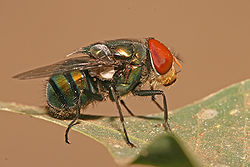
\includegraphics[width=6cm]{blow_fly.jpg}
\end{center}
\btVFill
\begin{flushright}
  \color{gray}
\tiny{Bialek, de Ruyer van Steveninck, Strong and other coworkers, late 1990s.}
\color{black}
\end{flushright}
\end{frame}



\begin{frame}{Difficulties with the classical approach.}
\begin{itemize}
\item Undersampling. 
\begin{itemize}
\item 100 ms words and 2 ms bins gives $2^{50}=1125899906842624$ words.
\item Lots of clever approaches to this, for example Nemenman et al. (PRE 2004, BMC Neuroscience 2007) where a cunning prior is used for $p(w_i)$.
\end{itemize}
\item Sampling bias.
\begin{itemize}
\item An even distribution will never give equal counts for each word,
  giving different $p(w_i)$.
\item Lots of clever approaches to this too, see Panzeri et al. (J Neurophys. 2007).
\end{itemize}
\end{itemize}
\end{frame}

\begin{frame}{Many fixes but still . . . }
\begin{itemize}
\item Neuron - neuron mutual information.
\item Maze - neuron mutual information.
\item Mutual information with multiple units.
\end{itemize}
\end{frame}


\begin{frame}{Approach 1: spike trains live in a metric space.}
\vskip 1cm  
Spike trains can be thought of as living in a metric space.
\vskip 1cm
\color{reddish}
\begin{center}
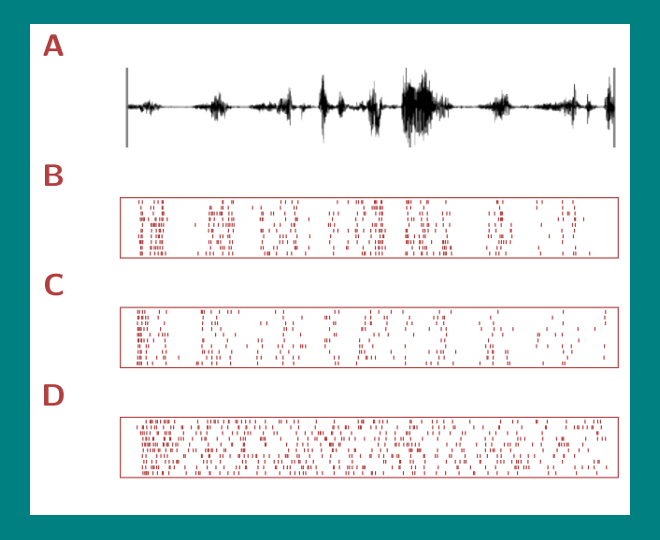
\includegraphics[width=5cm]{SpikeTrains.png}
\end{center}

  \btVFill
  \begin{flushright}
    \color{gray}
    \tiny{Jonathan Victor}
    \color{black}
\end{flushright}
\end{frame}


\begin{frame}{Approach 2: Kozachenko-Leonenko estimator.}
\vskip 3cm
  Here we will use a Kozachenko-Leonenko estimator.

  \btVFill
  \begin{flushright}
    \color{gray}
    \tiny{Kraskov, St\"{o}bauer and Grassberger (PRE 2004)}
    \color{black}
\end{flushright}
\end{frame}


\begin{frame}{A dart board}
\color{reddish}
\begin{center}
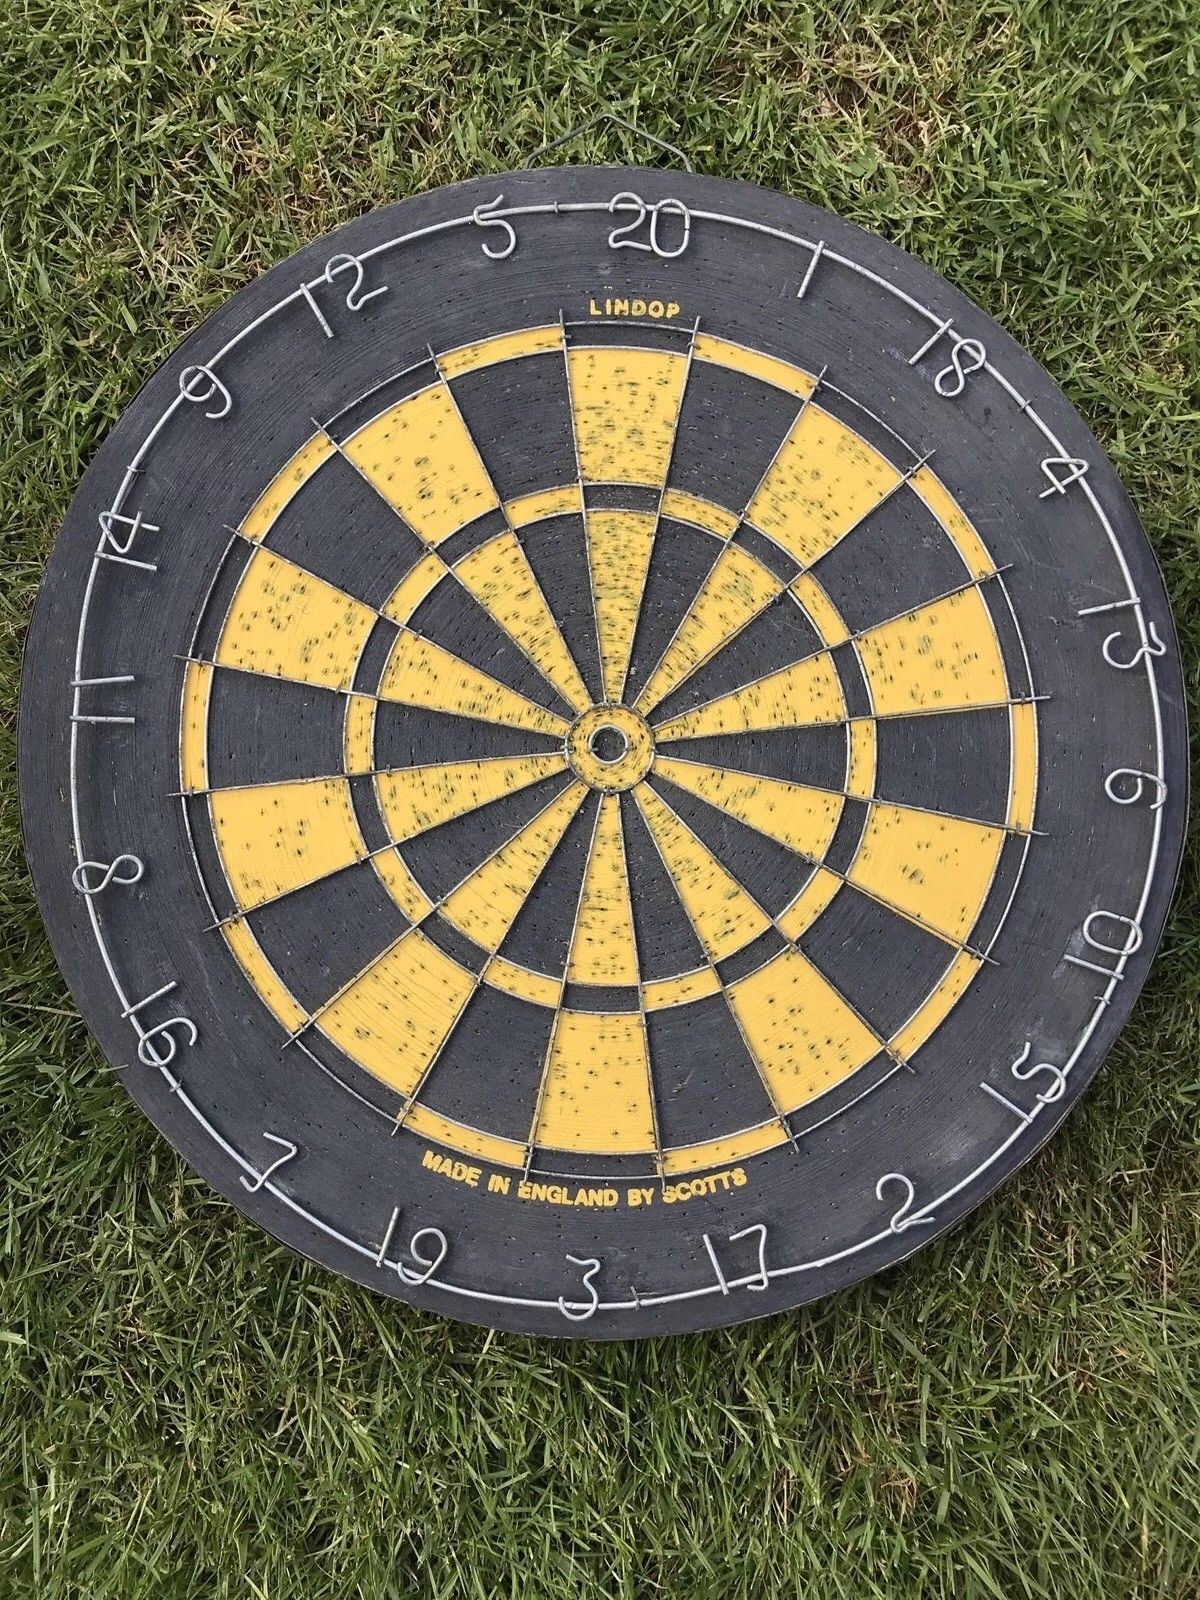
\includegraphics[width=4cm]{dart_board.jpg}
\end{center}
\color{black}
\btVFill
\color{gray}
\flushleft{\tiny{photo from ebay (\pounds 4.20 +p.p.)}}
\color{black}
\end{frame}

\begin{frame}{Probability mass function}
\color{reddish}
\begin{center}
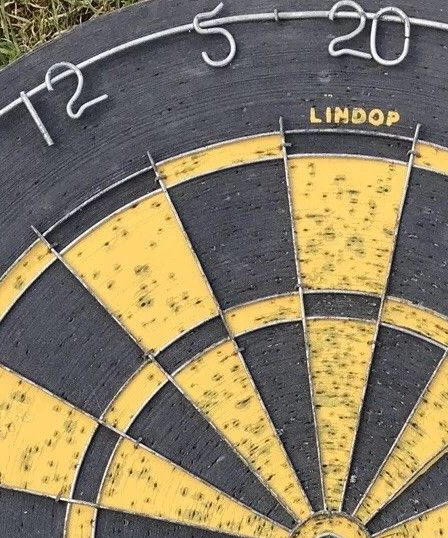
\includegraphics[width=4cm]{dart_board_zoom.png}
\end{center}
\begin{center}
\color{black}
$p(\mathbf{x})$ is the mass function
\end{center}
\color{black}
\end{frame}


\begin{frame}{Probability mass function}
\begin{center}
\includegraphics[width=4cm]{dart_board_region.png}
\end{center}
\color{dark}
$$\mbox{prob}(\mbox{dart lands in }B)=\int_B p(\mathbf{x})dV$$
\color{black}
\end{frame}


\begin{frame}{Estimating using the number of holes}
\color{reddish}
\begin{center}
\includegraphics[width=4cm]{dart_board_region.png}
\end{center}
\color{dark}
$$\langle \mbox{number of holes in }B\rangle \approx \int_B p(\mathbf{x})dV \times (\mbox{total number of holes})$$
\color{black}
where the total volume is normalized.
\end{frame}

\begin{frame}{Estimating the probability mass function}
\color{black}
If the mass function varies slowly:
\color{dark}
$$\int_B p(\mathbf{x})dV\approx p(\mathbf{x}_0) \times \mbox{vol}\,B$$
\color{black}
where $\textbf{x}_0$ is a point, for example, in the middle of $B$ where we are interested in. Now
\color{dark}
$$\mbox{number of holes in }B \approx p(\mathbf{x}_0) \times \mbox{vol}\,B \times (\mbox{total number of holes})$$
\color{black}
\end{frame}


\begin{frame}{Estimating using the number of holes}
\color{dark}
$$p(x_0)\approx\frac{\#B}{n\times \mbox{vol}\,B}
$$
\color{black}
where $n$ is the total number of points and $\#B$ is the number of points in $B$.
\color{reddish}
\begin{center}
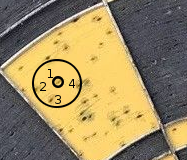
\includegraphics[width=4cm]{dart_board_zoom_ball.png}
\end{center}
\color{black}
so in this case
\color{dark}
$$p(\circ)=\frac{4}{n\mbox{vol}\,B}$$
\end{frame}


\begin{frame}{Estimating using the number of holes}
\color{dark}
$$p(x_0)\approx\frac{\#B}{n\times \mbox{vol}\,B}$$
\color{black}
Using this to find the mutual information gives a \textsl{Kozachenko-Leonenko} estimator.
\end{frame}

\begin{frame}{Kozachenko-Leonenko estimators are very good}
\color{reddish}
\begin{center}
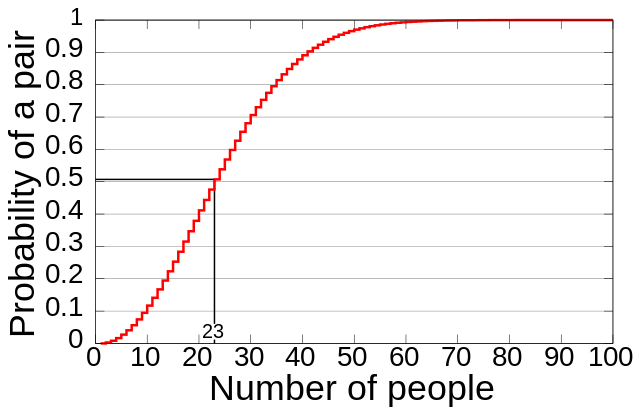
\includegraphics[width=6cm]{Birthday_Paradox.png}
\end{center}
\color{black}
\btVFill
\color{gray}
\flushleft{\tiny{graph from wikipedia article on the birthday paradox}}
\color{black}
\end{frame}



\begin{frame}{Problem}
\color{black}
How do we work out the volume in the space of spike trains? We have no coordinates $xyz$ to do
\color{dark}
$$\mbox{vol}\,B=\int_B dxdydz$$
\end{frame}


\begin{frame}{Problem}
\color{black}
How do we work out the volume in the space of spike trains? We have no coordinates $xyz$ to do
\color{dark}
$$\mbox{vol}\,B=\int_B dxdydz$$
\color{black}
Even if we had coordinates would we want to use them?
\end{frame}



\begin{frame}{Use the mass function as a measure!}
\color{dark}
$$\mbox{vol}\,B=\int_B p(\mathbf{x}) dV$$
\color{black}
A volume: 
\begin{itemize}
\item $A\subset B$ implies $\mbox{vol}\,A<\mbox{vol}\,B$.
\item $A\cap B=\phi$ implies $\mbox{vol}\,A\cup B<\mbox{vol}\,A+\mbox{vol}\,B$.
\end{itemize}
\end{frame}


\begin{frame}{Use the mass function as a measure!}
\color{reddish}
\begin{center}
\includegraphics[width=4cm]{dart_board_big_20.png}
\end{center}
\color{dark}
$$\mbox{vol}\,B=\int_B p(\mathbf{x}) dV$$
\color{black}
\end{frame}



\begin{frame}{Volume by counting holes}
\color{dark}
$$\mbox{vol}\,B=\int_B p(\mathbf{x}) dV\approx \frac{\mbox{number of holes in }B}{\mbox{total number of holes}}$$
\end{frame}

\begin{frame}{Volume by counting holes}
\color{reddish}
\begin{center}
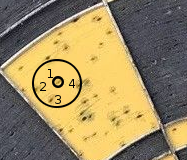
\includegraphics[width=4cm]{dart_board_zoom_ball.png}
\end{center}
\color{black}
A ball with volume $h/n$ around the circled point, where $n$ is the total number of holes and $h=4$.
\end{frame}


\begin{frame}{Metric}
To make a ball you need a metric; not to measure the radius since the
size is being defined by the volume, but to define \lq{}the nearest
$h$ points\rq{}.
\color{reddish}
\begin{center}
\color{reddish}
% GNUPLOT: LaTeX picture with Postscript
\begingroup
  \makeatletter
  \providecommand\color[2][]{%
    \GenericError{(gnuplot) \space\space\space\@spaces}{%
      Package color not loaded in conjunction with
      terminal option `colourtext'%
    }{See the gnuplot documentation for explanation.%
    }{Either use 'blacktext' in gnuplot or load the package
      color.sty in LaTeX.}%
    \renewcommand\color[2][]{}%
  }%
  \providecommand\includegraphics[2][]{%
    \GenericError{(gnuplot) \space\space\space\@spaces}{%
      Package graphicx or graphics not loaded%
    }{See the gnuplot documentation for explanation.%
    }{The gnuplot epslatex terminal needs graphicx.sty or graphics.sty.}%
    \renewcommand\includegraphics[2][]{}%
  }%
  \providecommand\rotatebox[2]{#2}%
  \@ifundefined{ifGPcolor}{%
    \newif\ifGPcolor
    \GPcolorfalse
  }{}%
  \@ifundefined{ifGPblacktext}{%
    \newif\ifGPblacktext
    \GPblacktexttrue
  }{}%
  % define a \g@addto@macro without @ in the name:
  \let\gplgaddtomacro\g@addto@macro
  % define empty templates for all commands taking text:
  \gdef\gplbacktext{}%
  \gdef\gplfronttext{}%
  \makeatother
  \ifGPblacktext
    % no textcolor at all
    \def\colorrgb#1{}%
    \def\colorgray#1{}%
  \else
    % gray or color?
    \ifGPcolor
      \def\colorrgb#1{\color[rgb]{#1}}%
      \def\colorgray#1{\color[gray]{#1}}%
      \expandafter\def\csname LTw\endcsname{\color{white}}%
      \expandafter\def\csname LTb\endcsname{\color{black}}%
      \expandafter\def\csname LTa\endcsname{\color{black}}%
      \expandafter\def\csname LT0\endcsname{\color[rgb]{1,0,0}}%
      \expandafter\def\csname LT1\endcsname{\color[rgb]{0,1,0}}%
      \expandafter\def\csname LT2\endcsname{\color[rgb]{0,0,1}}%
      \expandafter\def\csname LT3\endcsname{\color[rgb]{1,0,1}}%
      \expandafter\def\csname LT4\endcsname{\color[rgb]{0,1,1}}%
      \expandafter\def\csname LT5\endcsname{\color[rgb]{1,1,0}}%
      \expandafter\def\csname LT6\endcsname{\color[rgb]{0,0,0}}%
      \expandafter\def\csname LT7\endcsname{\color[rgb]{1,0.3,0}}%
      \expandafter\def\csname LT8\endcsname{\color[rgb]{0.5,0.5,0.5}}%
    \else
      % gray
      \def\colorrgb#1{\color{black}}%
      \def\colorgray#1{\color[gray]{#1}}%
      \expandafter\def\csname LTw\endcsname{\color{white}}%
      \expandafter\def\csname LTb\endcsname{\color{black}}%
      \expandafter\def\csname LTa\endcsname{\color{black}}%
      \expandafter\def\csname LT0\endcsname{\color{black}}%
      \expandafter\def\csname LT1\endcsname{\color{black}}%
      \expandafter\def\csname LT2\endcsname{\color{black}}%
      \expandafter\def\csname LT3\endcsname{\color{black}}%
      \expandafter\def\csname LT4\endcsname{\color{black}}%
      \expandafter\def\csname LT5\endcsname{\color{black}}%
      \expandafter\def\csname LT6\endcsname{\color{black}}%
      \expandafter\def\csname LT7\endcsname{\color{black}}%
      \expandafter\def\csname LT8\endcsname{\color{black}}%
    \fi
  \fi
  \setlength{\unitlength}{0.0500bp}%
  \begin{picture}(4320.00,3024.00)%
    \gplgaddtomacro\gplbacktext{%
      \csname LTb\endcsname%
      \put(682,790){\makebox(0,0)[r]{\strut{}-8}}%
      \put(682,1132){\makebox(0,0)[r]{\strut{}-6}}%
      \put(682,1475){\makebox(0,0)[r]{\strut{}-4}}%
      \put(682,1817){\makebox(0,0)[r]{\strut{}-2}}%
      \put(682,2160){\makebox(0,0)[r]{\strut{} 0}}%
      \put(682,2502){\makebox(0,0)[r]{\strut{} 2}}%
      \put(820,484){\makebox(0,0){\strut{} 0}}%
      \put(1440,484){\makebox(0,0){\strut{} 0.1}}%
      \put(2059,484){\makebox(0,0){\strut{} 0.2}}%
      \put(2678,484){\makebox(0,0){\strut{} 0.3}}%
      \put(3297,484){\makebox(0,0){\strut{} 0.4}}%
      \put(3917,484){\makebox(0,0){\strut{} 0.5}}%
      \put(176,1731){\rotatebox{-270}{\makebox(0,0){\strut{}field strength}}}%
      \put(2368,154){\makebox(0,0){\strut{}time (ms)}}%
    }%
    \gplgaddtomacro\gplfronttext{%
    }%
    \gplbacktext
    \put(0,0){\includegraphics{two_erps}}%
    \gplfronttext
  \end{picture}%
\endgroup

\end{center}
\end{frame}


\begin{frame}{Oh no}
\color{dark}
$$p(\mathbf{x}_0)\approx\frac{\#B}{n\times \mbox{vol}\,B}=\frac{h}{nh/n}=1$$
\color{black}
and using this meaure gives $H(X)=0$; in fact the
  differential entropy is not well-defined. However the
  mutual information is!
\end{frame}


\begin{frame}{Mutual infomation}
\color{dark}
$$I(X,Y)=H(Y)-H(Y|X)$$ 
\color{black}
has two probability distributions: $p_Y(y)$ and
  $p_{Y|X}(y|x)$.
\vskip 1cm
IDEA: use one to estimate volume, the other can then
  be estimated by counting!
\end{frame}


\begin{frame}{Idea}
  \vskip 1cm
Consider the case where $Y$ takes values on a metric space (\color{reddish}spike trains!\color{black})and $X$ on a discrete space (\color{reddish}which song?\color{black}).
\color{black}
\begin{center}
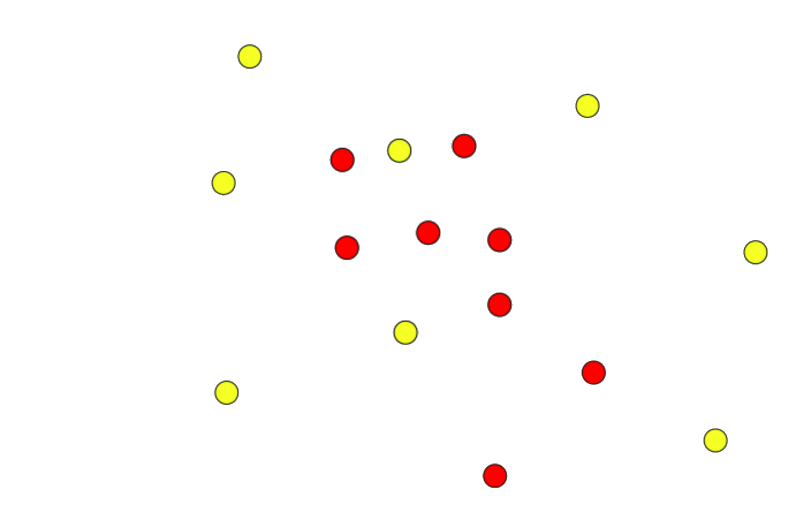
\includegraphics[width=6cm]{dots_simple.png}
\end{center}
\end{frame}



\begin{frame}{Idea}
  \vskip 1cm
Consider the case where $Y$ takes values on a metric space and $X$ on a discrete space.
  \vskip 1cm
  Use $p_Y(y)$ to estimate volume, a ball of radius $h$ has $h$ points in it, corresponding to any $X$ value.
\begin{center}
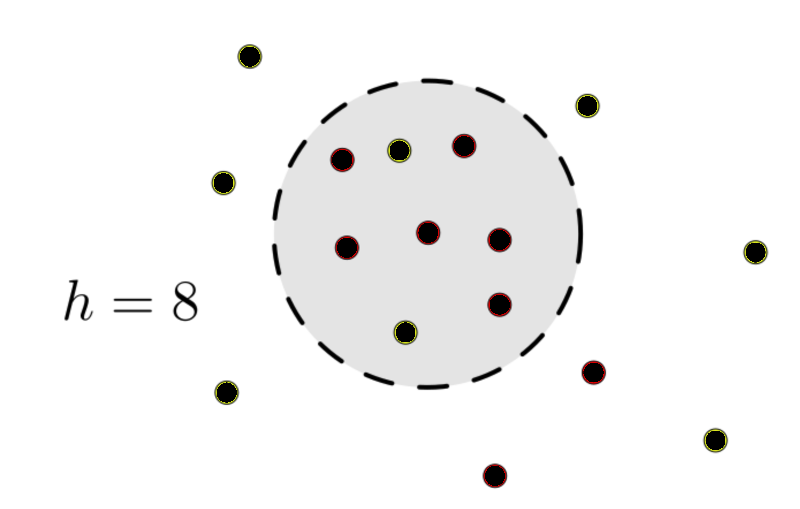
\includegraphics[width=6cm]{dots_black.png}
\end{center}
\end{frame}


\begin{frame}{Idea}
  \vskip 1cm
Consider the case where $Y$ takes values on a metric space and $X$ on a discrete space.
  \vskip 1cm
  Estimate $p_{Y|X}(y|x)$ by counting points: $p_{Y|X}(y|x)$ is estimated by counting the $y$ points in the ball corresponding to $X=x$.  
\color{black}
\begin{center}
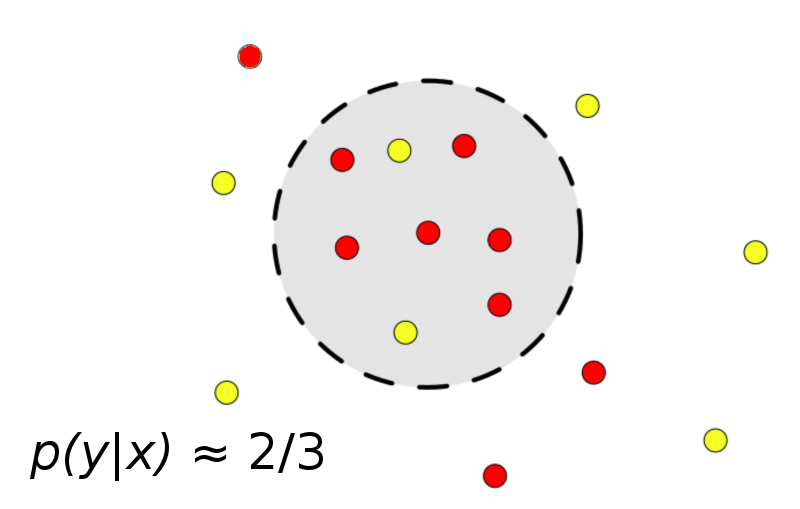
\includegraphics[width=6cm]{dots_prob.png}
\end{center}
\end{frame}


\begin{frame}{Formula}
This is for the case where $X$ is a discrete random variable and
everything exciting is happening in $Y$ space.
\color{dark}
$$I(X,Y)=\frac{1}{n}\sum_{y_i}\log_2{\frac{n_s\#_{y_i}B(y_i)}{h}}$$
\color{black} where $B(y_i)$ is the ball around $y$ and $\#_y{B(y)}$
  is the number of points in that correspond to the same $X$ value as
  $y$. $n_s$ is the number of stimuli.
\end{frame}


\begin{frame}{Formula}
\color{dark}
$$I(X,Y)=\frac{1}{n}\sum_{y_i}\log_2{\frac{n_s \#_{y_i}B(y_i)}{h}}$$
\color{black}
\begin{center}
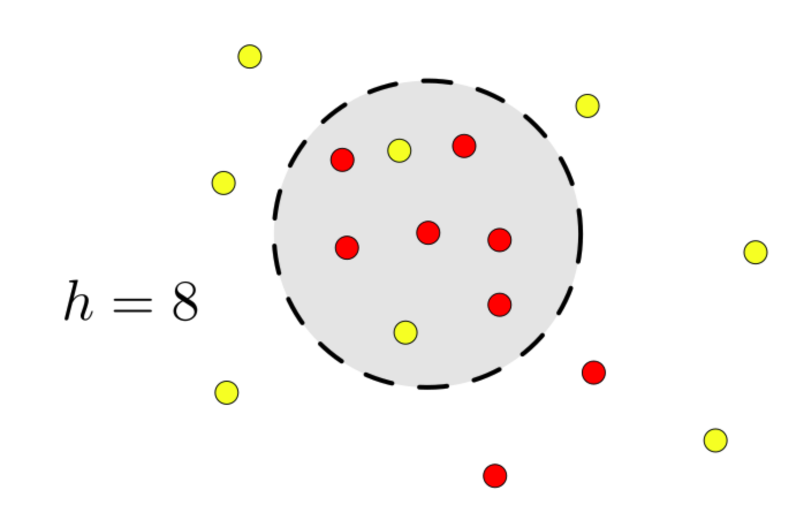
\includegraphics[width=6cm]{dots.png}
\end{center}
\end{frame}


\begin{frame}{h}

  There are two approximations:
  \color{dark}
$$\int_B p(x)dV \approx \# B\times \mbox{vol}\,B$$
\color{black}
  and
\color{dark}
  $$\int_B p(x)dV \approx \mbox{V}\times p(x_0)$$ 
\color{black}
The first approximation gets better if the volume is bigger, the
second gets worse; the correct choice of $h$ is a compromize between
these two. There is actually an approach to picking $h$ that
seems to work, based on the bias.
\end{frame}


\begin{frame}{Another formula}
\color{dark}
$$I(X,Y)=\frac{1}{n}\sum_{i=1}^n\log_2{\frac{n\#[C(u_i,v_i)]}{h^2}}$$
\color{black}
with $C(u_i,v_i)=C_U(u_i,v_i)\cup C_V(u_i,v_i)$
\begin{flushright}
  \setlength{\unitlength}{0.0500bp}%
  \begin{picture}(5040.00,3528.00)%
      \put(855,1818){\rotatebox{-270}{\makebox(0,0){\strut{}$V$}}}%
      \put(2519,154){\makebox(0,0){\strut{}$U$}}%
      \put(2400,3600){\makebox(0,0)[l]{\strut{}$C_U$}}%
      \put(4200, 1675){\makebox(0,0)[l]{\strut{}$C_V$}}%
      \put(2250,3400){\makebox(0,0)[l]{\strut{}$\overbrace{\;\,\qquad}$}}
      \put(3950,1665){\makebox(0,0)[l]{\strut{}$\left.\rule{0cm}{0.9cm}\right\}$}}
    \put(0,0){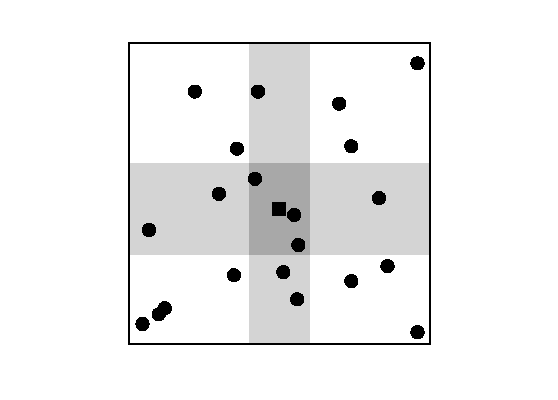
\includegraphics{NECO-07-18-3199-Figure-1.eps}}%
  \end{picture}%
\end{flushright}
\end{frame}


\begin{frame}{Fictive data}
\color{reddish}
\begin{center}
\begin{center}
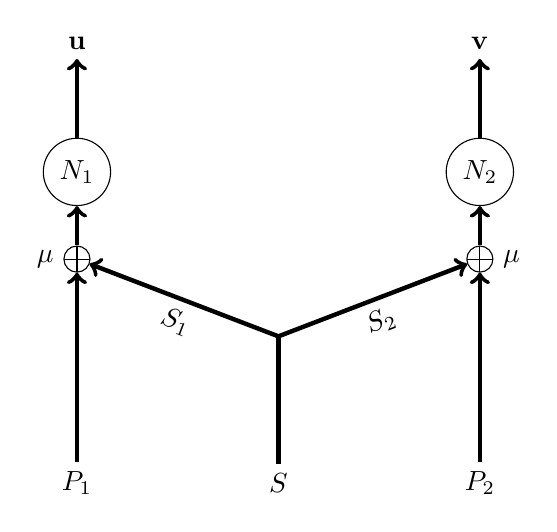
\begin{tikzpicture}[cross/.style={path picture={ 
  \draw[black] (path picture bounding box.south) -- (path picture
  bounding box.north) (path picture bounding box.west) -- (path
  picture bounding box.east); }}] \node (neuron1) at (0,0)
  [circle,draw] {$N_1$}; \node (middle)[right = 2cm of neuron1]{};
  \node (neuron2) [circle, right = 2cm of middle,draw] {$N_2$}; \node
  (a)[below = 1.5cm of neuron1]{}; \node (b)[below = 1.84cm of
    middle]{}; \node (c)[below = 1.5cm of neuron2]{};

\node (mu1)[circle,cross,below  = 0.5cm of neuron1,draw]{};
\node (mu2)[circle,cross,below  = 0.5cm of neuron2,draw]{};
\node (mumu1)[left = 0.0cm of mu1]{$\mu$};
\node (mumu2)[right = 0.0cm of mu2]{$\mu$};


\draw [ultra thick,->] (mu1)--(neuron1);
\draw [ultra thick,->] (mu2)--(neuron2);


\draw [ultra thick,->](b.center)--(mu1) node(s1)[midway, below, sloped]{$S_1$};
\draw [ultra thick,->](b.center)--(mu2) node(s2)[midway, below, sloped]{$S_2$};
\node(p1) [below=1.5cm of a]{$P_1$};
\node(s) [below=1.5cm of b]{$S$};
\node(p2) [below=1.5cm of c]{$P_2$};
\draw [ultra thick,->] (p1)--(mu1);
\draw [ultra thick](s)--(b.center);
\draw [ultra thick,->](p2)--(mu2);
\node (u) [above = 1cm of neuron1]{$\mathbf{u}$};
\node (v) [above = 1cm of neuron2]{$\mathbf{v}$};
\draw [ultra thick,->](neuron1)--(u);
\draw [ultra thick,->](neuron2)--(v);

\end{tikzpicture}
\end{center}
\end{center}
\end{frame}


\begin{frame}{van Rossum metric}
\begin{center}
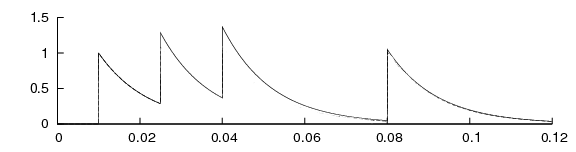
\includegraphics[width=9cm]{filtered.png}
\end{center}
Spike trains mapped to functions and a metric on the space of functions induces a metric on the spike train space.
\btVFill
\color{gray}
\begin{flushright}
\tiny{van Rossum (Neural Comp. 2001)}
\end{flushright}
\end{frame}



\begin{frame}{Result}
\color{reddish}
\begin{center}
  \setlength{\unitlength}{0.0500bp}%
  \begin{picture}(5040.00,3528.00)%
        \put(946,901){\makebox(0,0)[r]{\strut{} 0}}%
      \put(946,1295){\makebox(0,0)[r]{\strut{} 0.2}}%
      \put(946,1688){\makebox(0,0)[r]{\strut{} 0.4}}%
      \put(946,2082){\makebox(0,0)[r]{\strut{} 0.6}}%
      \put(946,2476){\makebox(0,0)[r]{\strut{} 0.8}}%
      \put(946,2869){\makebox(0,0)[r]{\strut{} 1}}%
      \put(946,3263){\makebox(0,0)[r]{\strut{} 1.2}}%
      \put(1078,484){\makebox(0,0){\strut{} 0}}%
      \put(1791,484){\makebox(0,0){\strut{} 0.2}}%
      \put(2504,484){\makebox(0,0){\strut{} 0.4}}%
      \put(3217,484){\makebox(0,0){\strut{} 0.6}}%
      \put(3930,484){\makebox(0,0){\strut{} 0.8}}%
      \put(4643,484){\makebox(0,0){\strut{} 1}}%
      \put(176,1983){\rotatebox{-270}{\makebox(0,0){\strut{}mutual information (bits)}}}%
      \put(2860,154){\makebox(0,0){\strut{}$\mu$}}%
        \put(1610,3140){\makebox(0,0)[l]{\strut{}new 200 s}}%
        \put(1610,2920){\makebox(0,0)[l]{\strut{}old 2000 s}}%
        \put(1610,2700){\makebox(0,0)[l]{\strut{}old 25000 s}}%
      \put(0,0){\includegraphics{NECO-07-18-3199-Figure-3.eps}}%
  \end{picture}
\end{center}
\end{frame}

\begin{frame}{Conclusion}
  \color{black}
  \begin{itemize}
  \item It works remarkably well!
  \item Does it work for functions?
  \item Does it do clustering?
    \item Does it do ICA?
  \item Are there applications to machine learning and data science?
    \end{itemize}
\end{frame}

\begin{frame}{The end}
  \color{black}
  References:
  \begin{itemize}
  \item \textsl{A kernel-based calculation of information on a metric space.}
    R. Joshua Tobin and Conor J. Houghton, Entropy 15 (2013)
    4540-4552.
  \item \textsl{Calculating mutual information for spike trains and other data
    with distances but no coordinates.} Conor Houghton, Royal Society
    Open Science, 2 (2015) 140391.
  \item \textsl{Calculating the mutual information between two spike trains.} Conor Houghton, Neural Computation (2019) 31:330-343.
    \end{itemize}
  Funding: the James S McDonnell Foundation.
  \begin{center}
THANK YOU!
\end{center}
\end{frame}



\end{document}

